\chapter{State of the art}
\label{chap2}

% Today micro-controllers and other embedded electronics are in almost everything we use. Because of this, ensuring the secure operation of these devices is critical. While much attention is directed towards software and firmware security, hardware security often goes overlooked. Particularly, hardware fault-injection (glitching) has repeatedly demonstrated its capability to bypass conventional security measures. Examples include bypassing cryptographic signature validation of firmware binaries \cite{hole_in_soc}, re-enabling hardware debug functionality on production/fused processors\cite{reenable_debug} and bypassing input validation of data that crosses trust boundaries between privilege levels\cite{qualcom}. To stop these glitch attacks, a number of countermeasures can be introduced. This project looks at the ones implemented by the OpenHW Group for their 'CV32E40S' RISC-V core\cite{cv32e40s_manual}, and how these security measures can be avoided entirely by instead running a dual-core RISC-V setup with lockstep. 
% After the discovery of the first glitch attack in 2002, many other examples have followed. These include bypassing cryptographic signature validation of firmware binaries \cite{hole_in_soc}. This was done using voltage glitching to bypass the verification of a firmware images signature. re-enabling hardware debug functionality on production/fused processors\cite{reenable_debug} and bypassing input validation of data that crosses trust boundaries between privilege levels\cite{qualcom}.

The RISC-V architecture has over recent years gained a lot of traction in both academia and industry due to its modular design and adaptability\cite{source2}. However, due to the nature of open source resources, RISC-V systems are often more susceptible to glitch attacks as hackers can research the ISA in depth to find errors. This was done in 2021 by two researchers\cite{isa_exploit}. What they found was that in the ISA there was never specified a base address for the \textit{Machine Trap Vector} (MTVEC) before booting up a RISC-V core. As the MTVEC is resposnsible for handling exceptions, this lead to an exploitable issue: If an attacker were to induce some exception during boot, it would be handled by the MTVEC. However, as the MTVEC had no base address (0x00000000) it would raise another exception. This then leads to an infinite exception loop which can be exploited. In addition to this vulnerability due to the availability of sensitive information, the actual chips made with the RISC-V architecture will still be susceptible to more common attacks like electromagnetic fault injection (EMFI) or voltage- and clock-glitching. 

% Often the security measures that are implemented aim at stopping one specific form of attack. Take for instance the example code shown in \autoref{fig:glitchable_code}. This code represents a secure boot process where first an image is fetched. The result code of the fetch operation is then checked to see whether the correct image was fetched, or if an error occurred. In the case of the latter, the program is stuck in in an infinite loop and if not the boot process can continue. From the figure one can observe that there exists a number of weak points that can be exploited. Because of this hardware designers implement things like \textit{Program Counter Hardening} (PCH) to check for instruction skips by comparing current and expected PC values, and \textit{Error Correcting Code} (ECC) to validate data integrity in registers. However, while these features would stop an attacker in this example, what if the attacker finds a way to boot with the wrong PC and start at the 'do\_boot' instruction? In this case we would need to develop a new form of protection with a greater fault detection coverage. Such a solution is discussed in this project in the form of a dual-core lockstep mechanism. 

% \begin{figure}[h!]
%     \centering
%     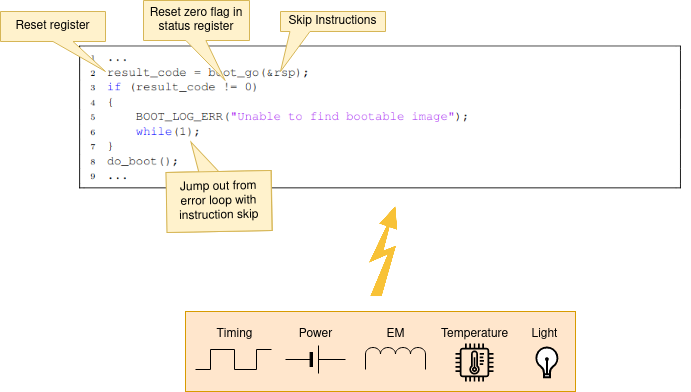
\includegraphics[width=0.75\textwidth]{docs/images/glitch_attack_whole_system.png}
%     \caption{Example of code that can be glitched with common attacks. \textit{Figure inspired by one found in “Fault Attacks on Secure Embedded Software:
% Threats, Design and Evaluation”, Bilgiday Yuce, Patrick Schaumont,
% Marc Witteman}}
%     \label{fig:glitchable_code}
% \end{figure}


 
%4. Scope of the Problem:

%System Vulnerabilities: An in-depth understanding of where and how glitches typically affect RISC-V cores is crucial. This entails both functional and performance impacts.
%Dual Core Strategy: Introducing a dual-core setup offers potential glitch protection via redundancy. However, the feasibility, overheads, synchronization mechanisms, and actual effectiveness of such a strategy need thorough examination.
%Protection Mechanisms: Beyond the mere introduction of dual cores, the strategies for detection of a glitch, switch-over mechanisms, and potential recovery strategies need to be explored.
%5. Objectives:

%The primary objectives for this project include:

%Conducting a vulnerability analysis of single-core RISC-V systems concerning glitches.
%Designing a dual-core RISC-V system prototype aiming for glitch protection.
%Evaluating the effectiveness of the dual-core setup in real-world scenarios and benchmark tests.
%Proposing additional countermeasures or strategies, if needed, to enhance glitch protection further.
%6. Significance:
%By addressing the problem defined, this project aims not only to enhance the reliability of RISC-V based systems but also to contribute to the broader realm of glitch protection in electronics. With the ever-increasing adoption of RISC-V in various applications, ensuring its robustness against glitches will be paramount for many industries.

